% Chapter 2. Literature review
% Writing rules: no first person, no "its", no "respectively", no colons or semicolons joining clauses,
% past tense for the methods and results of specific studies, present tense for established facts and figures.

\chapter{Literature Review}
\label{ch:review}

\section{Mixed-composition perovskite solar cells}
\label{sec:mixed}

\subsection{Record single-junction cells}

Metal halide perovskites have the formula ABX$_3$, where A is a monovalent cation, B is a divalent metal and X is a halide. The record single-junction perovskite cells of the past decade have used mixed compositions, with more than one cation on the A site or more than one halide on the X site. \citet{Jeon2015} mixed formamidinium lead iodide with methylammonium lead bromide and stabilized the black phase of the formamidinium-rich film, which raised the efficiency above 18\,\%. \citet{Saliba2016} added cesium to this mixture. The resulting triple-cation films crystallized more reproducibly and reached a stabilized efficiency of 21.1\,\%. Later work kept the formamidinium-rich composition and improved the film and the interfaces. \citet{Jeong2021} replaced part of the iodide with the formate pseudo-halide, and \citet{Min2021} grew an atomically coherent interlayer on the SnO$_2$ electrode. Both studies exceeded 25\,\%. \citet{Park2023} controlled the film growth with volatile alkylammonium chlorides and obtained a certified efficiency of 26.08\,\%. The certified record now stands at about 27\,\% \citep{NREL2026}.

These record compositions all contain organic A-site cations. Methylammonium and formamidinium are volatile, and the films decompose at the temperatures used for processing and testing. Thermal stability therefore remains the main weakness of hybrid perovskite cells.

\subsection{All-inorganic mixed-halide perovskites}

Replacing the organic cation with cesium removes the volatile component. \citet{Eperon2015} reported the first \cpi{} solar cells, with an efficiency of 2.9\,\%. \citet{Wang2019} stabilized the black phase of \cpi{} and exceeded 18\,\%, and \citet{Mali2023} reached more than 21.5\,\% with a phase heterojunction of two black polymorphs. These efficiencies remain below those of the hybrid cells.

Iodide and bromide mix on the X site of CsPb(I$_{1-x}$Br$_x$)$_3$ over the whole composition range. The mixture is a substitutional solid solution, so a film of a given $x$ is a single crystalline phase and not a composite of CsPbI$_3$ and CsPbBr$_3$ grains. The film is still polycrystalline, with grains of the same mixed composition. Because the halides share one sublattice, the band gap, the lattice parameter and the phase stability change continuously with $x$. \citet{Sutton2016} tuned the band gap from 1.73 to 2.3~eV across the series and found that the bromide-rich compositions remained stable at high temperature. \citet{Beal2016} reported that CsPbBr$_{1}$I$_{2}$, with a band gap of 1.92~eV, retained the black phase more readily than \cpi{}. A single-phase mixture is not guaranteed under operation, however. \citet{Hoke2015} observed that illumination separated mixed-halide hybrid perovskites into iodide-rich and bromide-rich domains, a process mediated by halide migration. The physics of the mixed crystal therefore differs from a simple average of the two end members.

\section{Tandem solar cells}
\label{sec:tandem}

A single absorber cannot use the whole solar spectrum. Photons with energy below the band gap pass through the absorber, and photons far above the band gap lose the excess energy as heat when the photogenerated carriers relax to the band edges. The detailed-balance analysis of \citet{Shockley1961} placed the maximum efficiency of a single junction at about 33\,\% under one sun, at a band gap of about 1.3~eV.

A tandem cell divides the spectrum between two absorbers (Fig.~\ref{fig:tandem}). The top cell has the wider band gap. The top cell absorbs the high-energy photons and transmits the low-energy photons to the bottom cell, which has the narrower band gap. Each photon is then absorbed by a cell whose band gap lies closer to the photon energy, which reduces both the transmission loss and the thermalization loss. \citet{DeVos1980} extended the detailed-balance analysis to stacked cells and showed that two junctions raise the limit above 40\,\% under one sun.

In the monolithic two-terminal design, the two cells are connected in series through a recombination layer. Electrons from one cell recombine in this layer with holes from the other cell, so the voltages of the two cells add and the same current flows through both. The current of the tandem is therefore limited by the weaker cell, and the band gaps must be chosen so that the two cells generate equal currents. For a silicon bottom cell with a band gap of 1.12~eV, \citet{Horantner2017} calculated that the optimum top-cell band gap lies near 1.7--1.8~eV.

\begin{figure}[htbp]
  \centering
  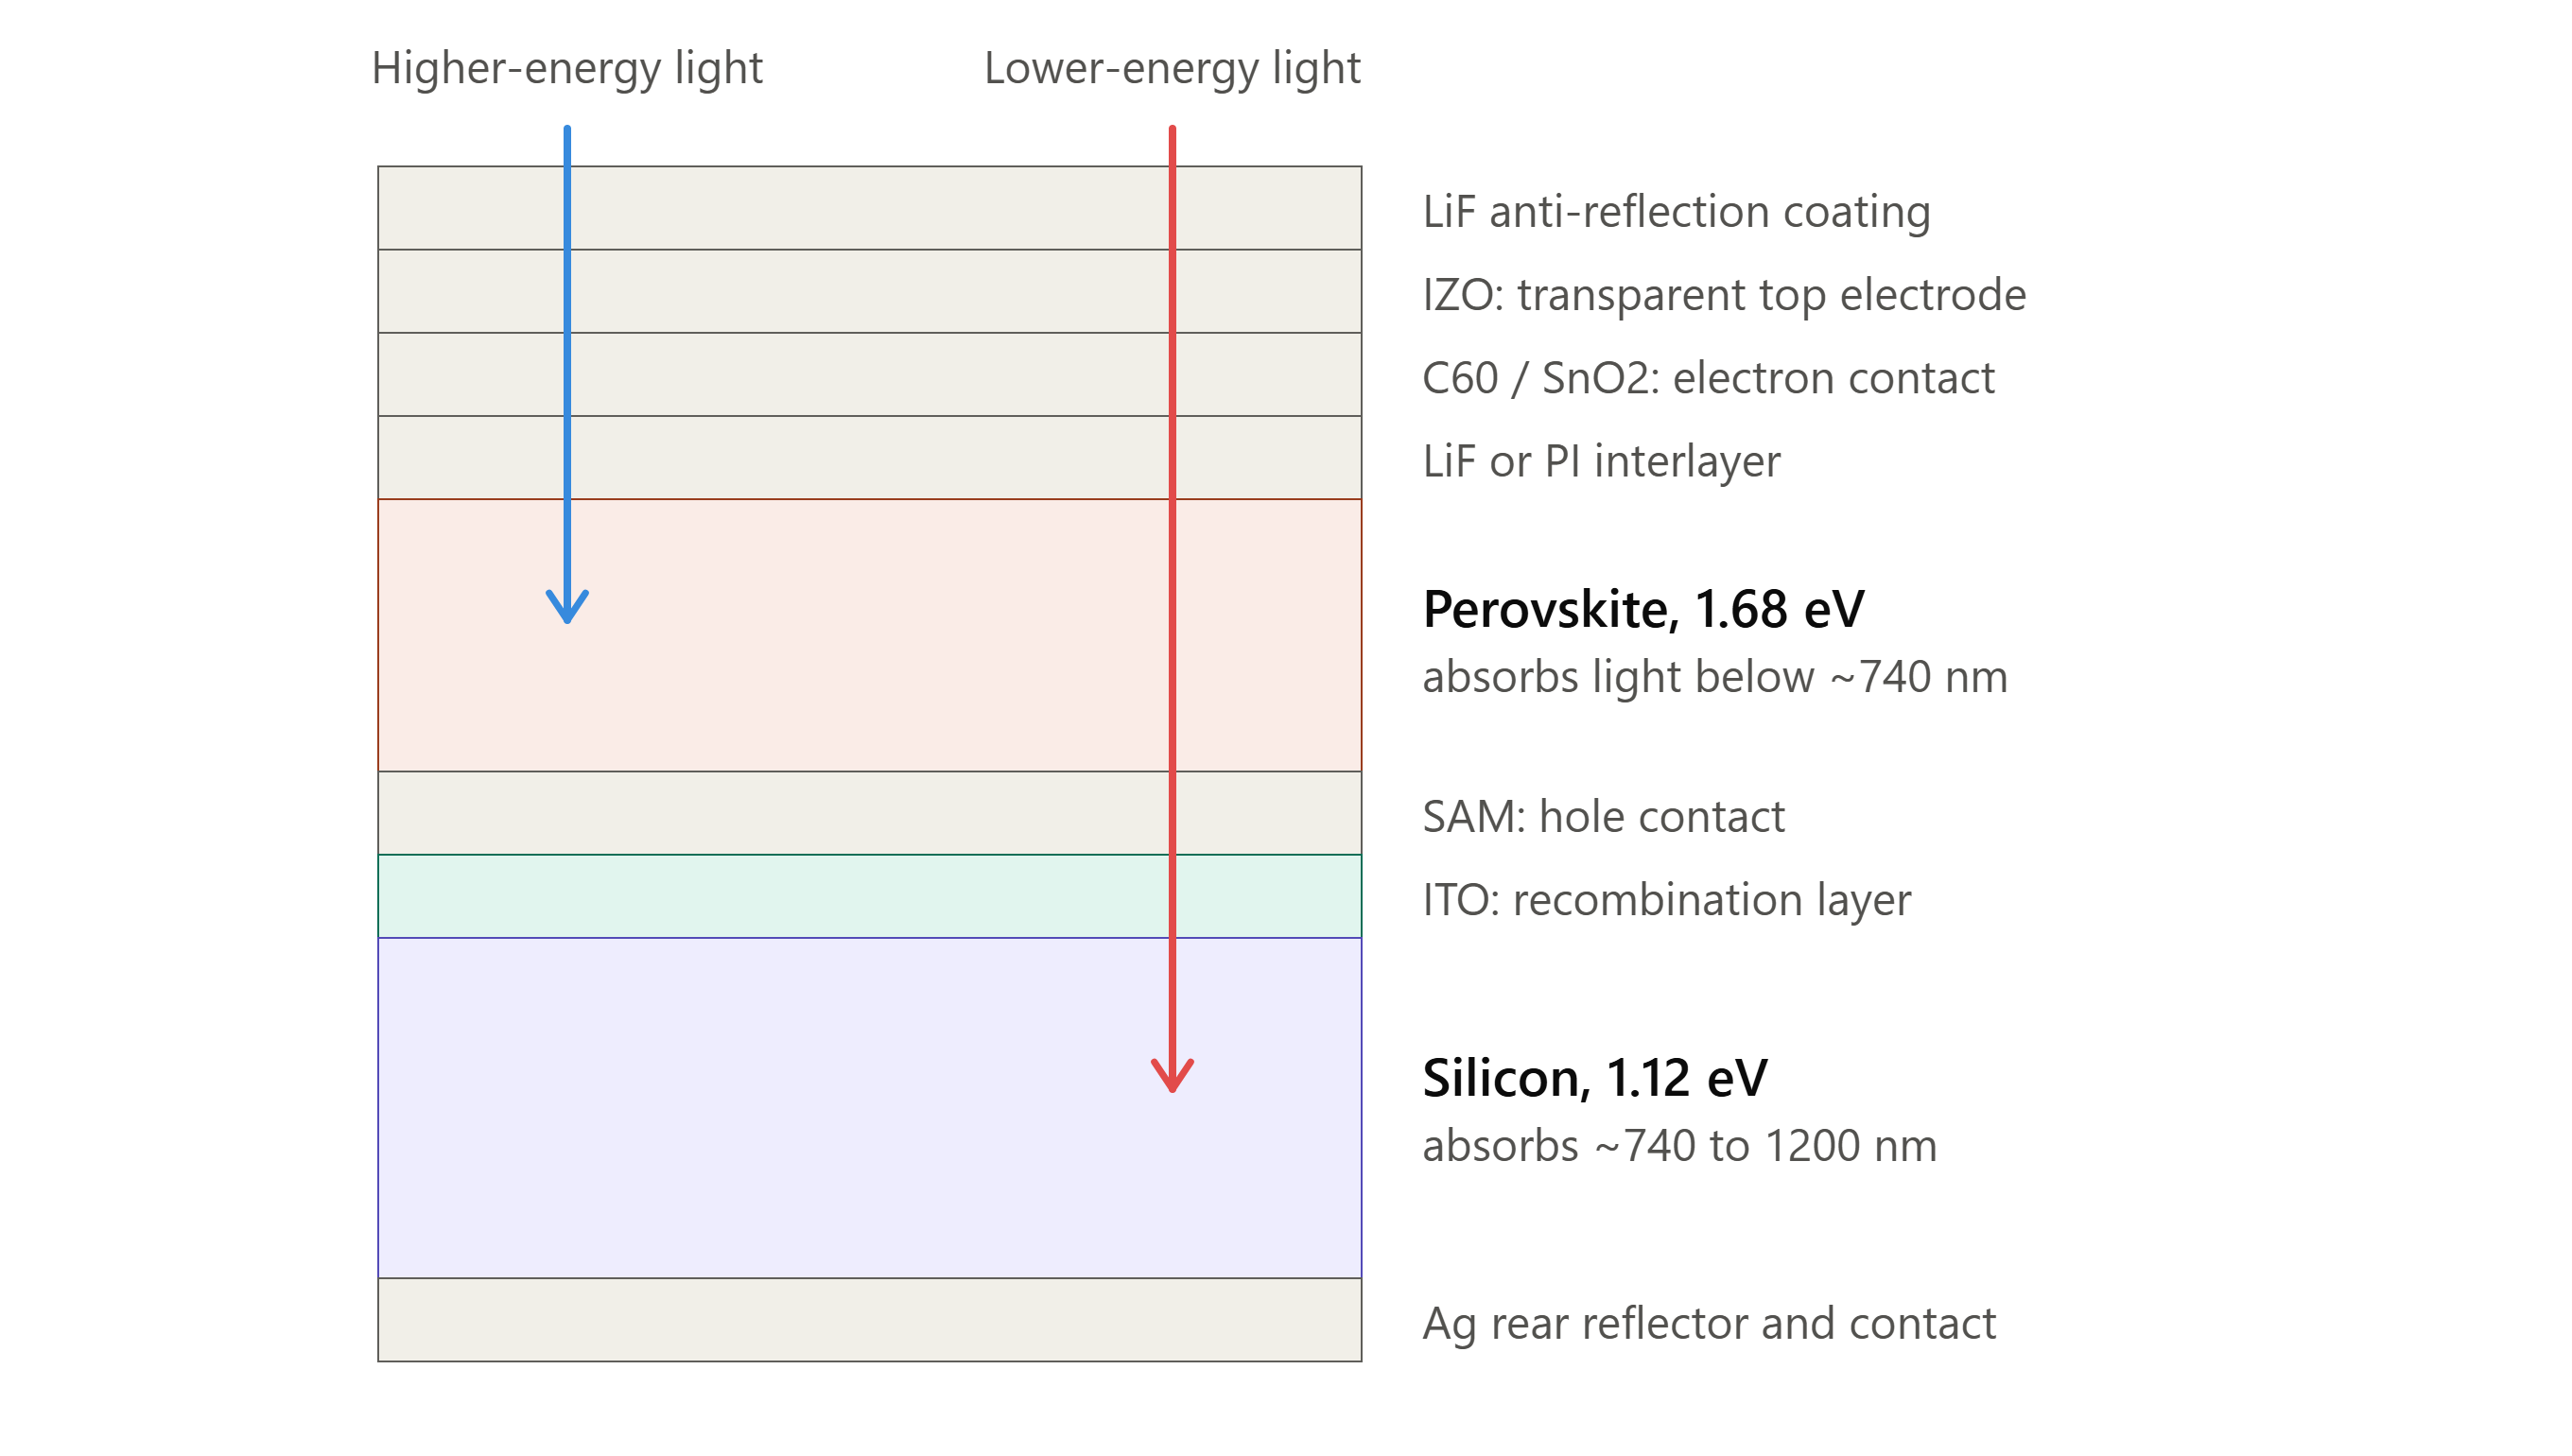
\includegraphics[width=0.8\linewidth]{perovskite_silicon_tandem_stack.png}
  \caption{Layer stack of a monolithic perovskite/silicon tandem cell. The perovskite top cell absorbs the high-energy light and transmits the low-energy light to the silicon bottom cell. The recombination layer connects the two cells in series.}
  \label{fig:tandem}
\end{figure}

Perovskites suit the top cell because the band gap can be tuned through the composition. \citet{AlAshouri2020} reported a perovskite/silicon tandem with an efficiency above 29\,\%, and \citet{Mariotti2023} reached a certified 32.5\,\% with a triple-halide top cell. Certified perovskite/silicon tandems now exceed 34\,\% \citep{NREL2026}. The record top cells still contain organic cations. The band gap of \cpi{}, about 1.7~eV, lies in the optimum range for a silicon bottom cell, and bromide substitution raises the gap further for other bottom cells \citep{Sutton2016,Beal2016}. All-inorganic mixed-halide perovskites are therefore candidate top cells that combine a suitable band gap with thermal stability.

\section{Phase stability of CsPbI$_3$}
\label{sec:phase}

\cpi{} has four polymorphs. Three of them, the cubic $\alpha$ phase, the tetragonal $\beta$ phase and the orthorhombic $\gamma$ phase, consist of corner-sharing PbI$_6$ octahedra. These three phases differ only by the tilt of the octahedra, and all three are black and photoactive. On cooling, $\alpha$ transforms to $\beta$ at about 533~K and $\beta$ transforms to $\gamma$ at about 448~K \citep{Marronnier2018}. These transformations are displacive and fast. The fourth polymorph, the $\delta$ phase, consists of chains of edge-sharing octahedra. The $\delta$ phase is yellow and has a band gap of about 2.8~eV, which is too wide for an efficient absorber \citep{Sutton2018}.

At room temperature, the stability of the four phases increases in the order $\alpha$, $\beta$, $\gamma$, $\delta$, and $\delta$ is the ground state. The phase diagram of the CsI--PbI$_2$ system (Fig.~\ref{fig:phase}) shows that $\alpha$-\cpi{} is stable only between 599 and 758~K and that $\delta$-\cpi{} is stable below 599~K \citep{vanHattem2023}. The $\beta$ and $\gamma$ phases do not appear on the equilibrium diagram, because neither is stable at any temperature. Black films are therefore made by annealing in the $\alpha$ range and cooling quickly. The fast tilt transitions then produce $\gamma$-\cpi{}, which is metastable with respect to $\delta$.

\begin{figure}[htbp]
  \centering
  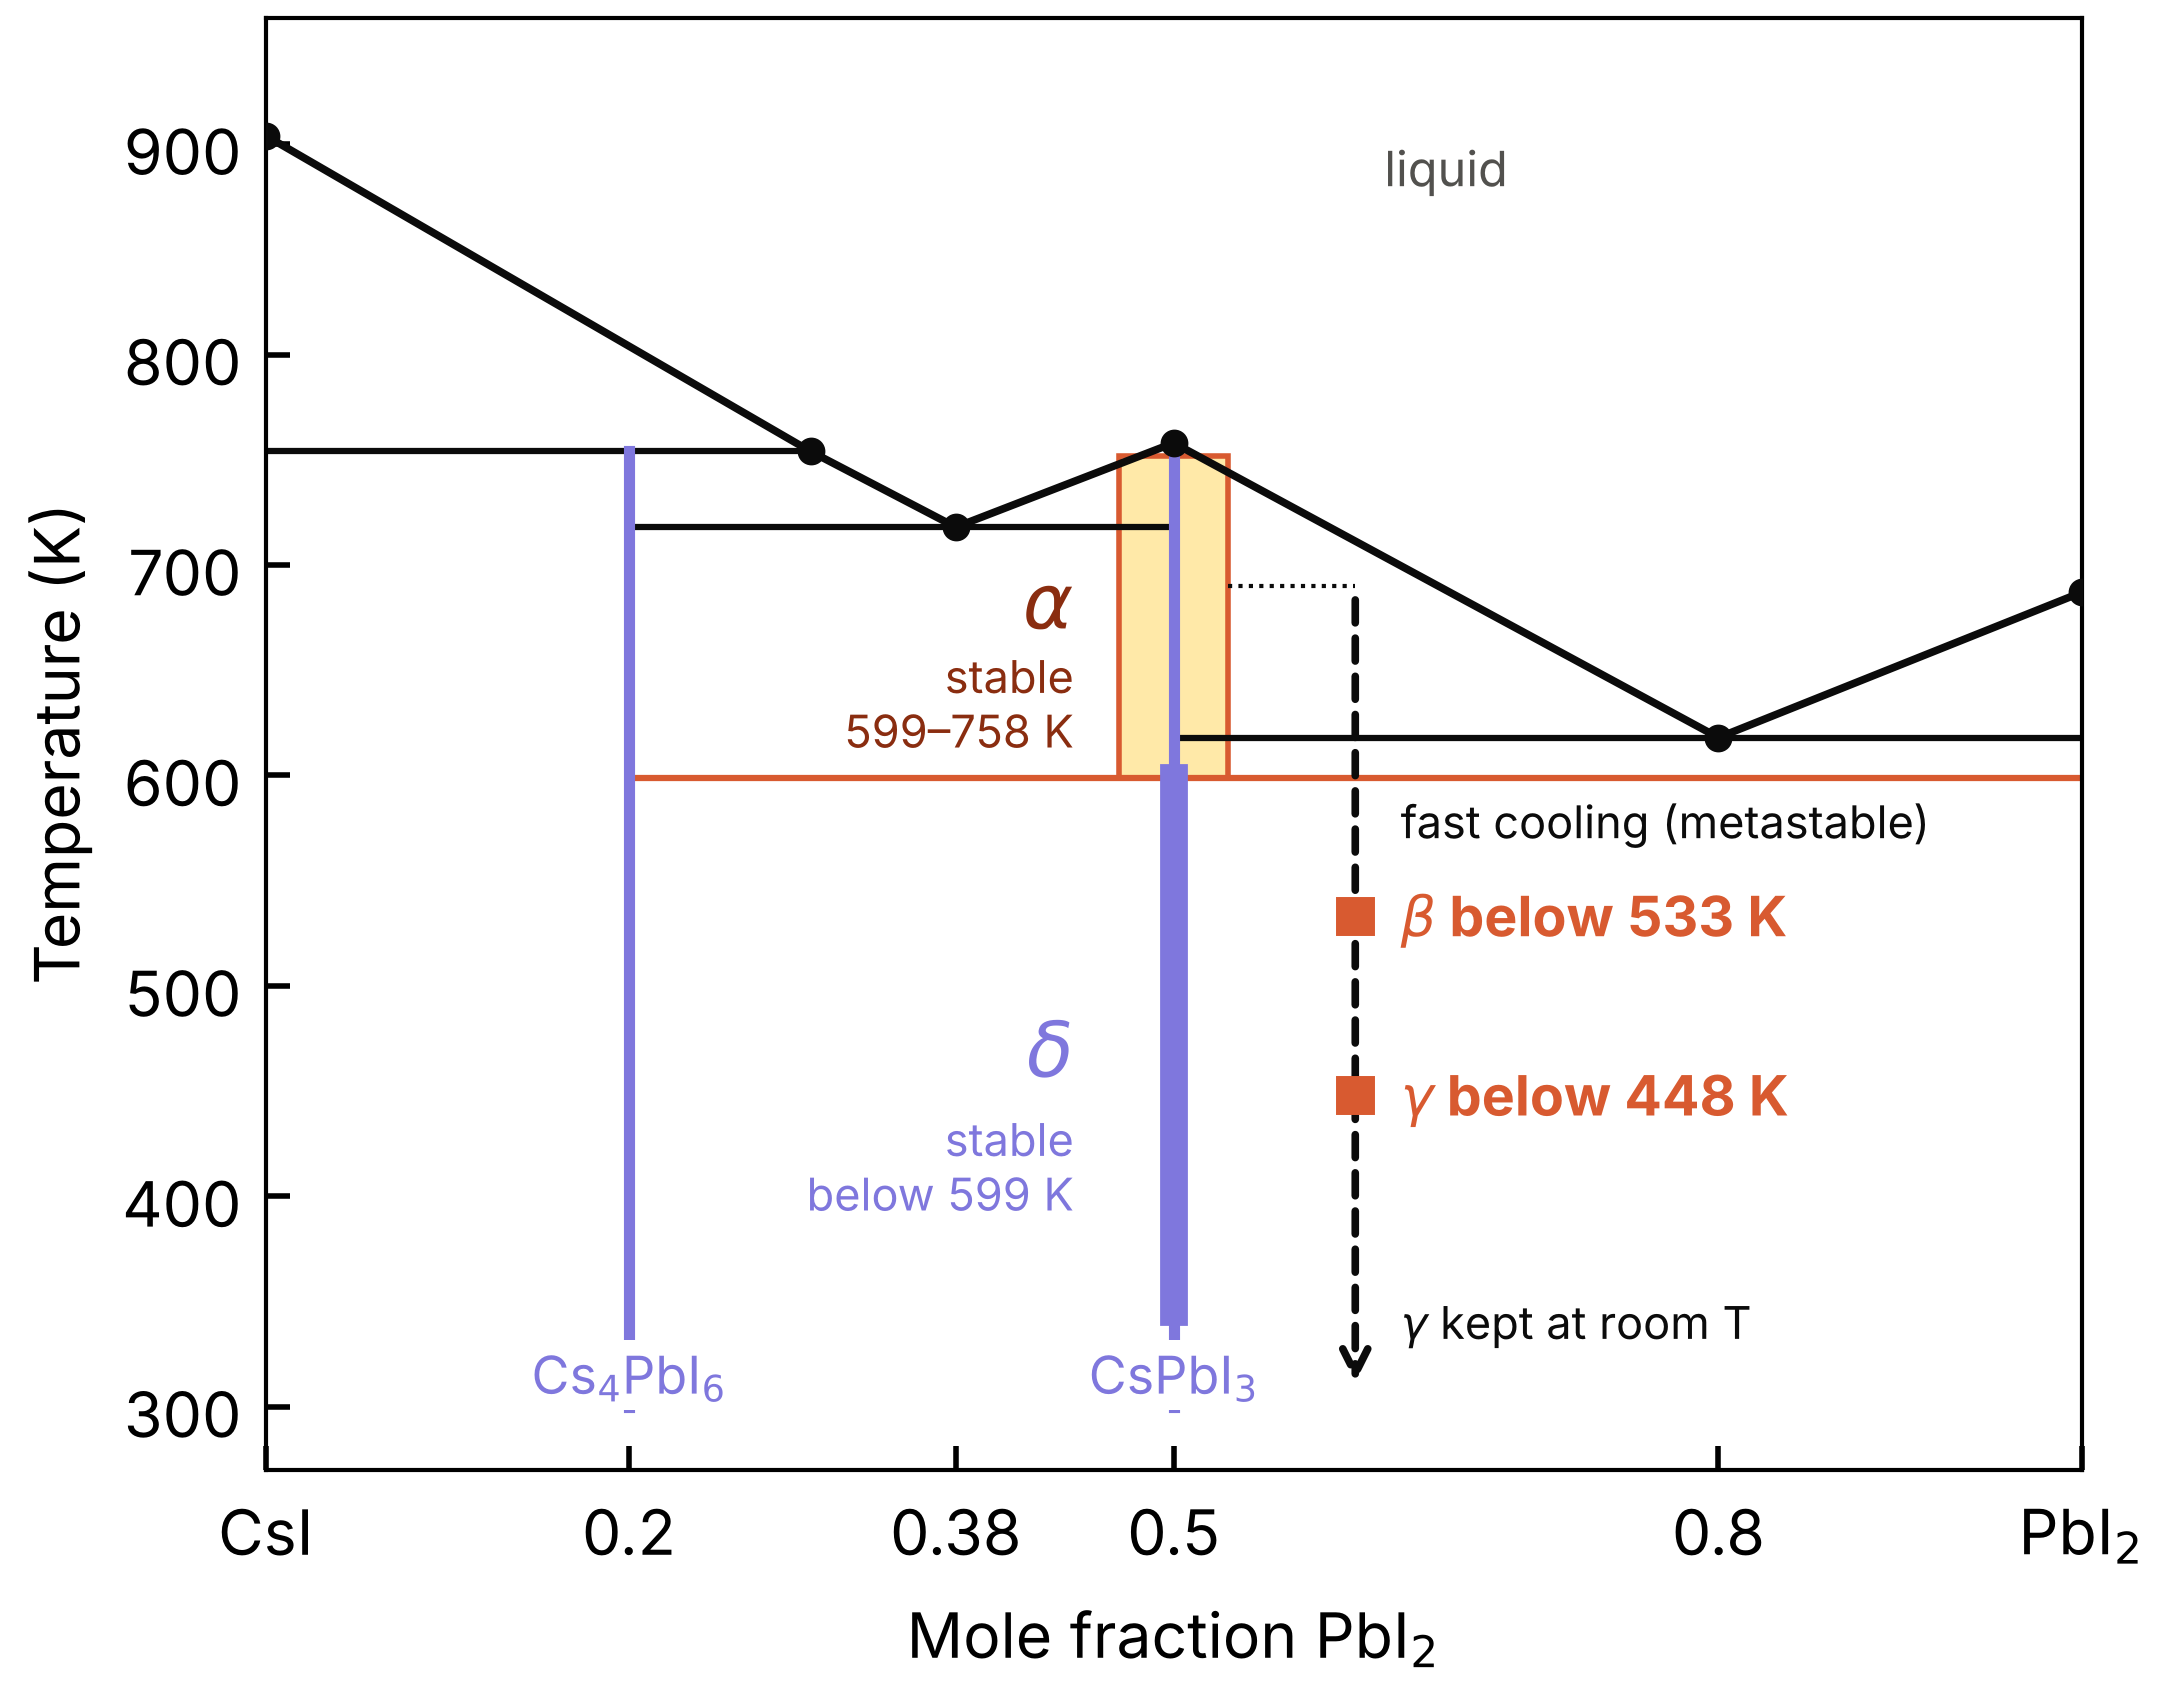
\includegraphics[width=0.75\linewidth]{phase_CsI_PbI2_phases.png}
  \caption{CsI--PbI$_2$ phase diagram, drawn from the data of \citet{vanHattem2023}. The $\alpha$ phase of CsPbI$_3$ is stable between 599 and 758~K and the $\delta$ phase below 599~K. The dashed path marks the metastable $\beta$ and $\gamma$ phases formed on fast cooling \citep{Marronnier2018}.}
  \label{fig:phase}
\end{figure}

At room temperature, $\gamma$-\cpi{} slowly transforms into the $\delta$ phase. This transformation rebuilds the octahedral network from corner sharing to edge sharing, so the transformation requires nucleation and long-range atomic rearrangement. Moisture accelerates the transformation. \citet{Steele2019} observed that black films exposed to humid air quickly turned yellow, and \citet{Le2023} attributed the moisture-induced transformation of \cpi{} nanoplates to surface halide vacancies.

\section{Strain and the black phase}
\label{sec:strain-phase}

Experiments have shown that tensile strain keeps \cpi{} in the black phase. \citet{Steele2019} annealed \cpi{} films on glass and indium tin oxide substrates at 330~$^\circ$C and cooled them. The substrate prevented the films from shrinking in the plane of the film, which left an in-plane biaxial tensile strain of about 1\,\%. The clamped films stayed black, whereas free nanocrystals scraped from the same films turned yellow below 230~$^\circ$C. \citet{Le2023} grew \cpi{} nanoplates on mica with a lattice mismatch that imposed in-plane tension. After one month, 56\,\% of the thin plates and 31\,\% of the thick plates remained in the black phase. \citet{Steele2021} also found that dopants which suppress the spontaneous strain of the tilted lattice stabilize the black phase.

The mechanism of this stabilization is less clear. Strain could act thermodynamically, by raising the energy of $\delta$ above that of $\gamma$, or kinetically, by raising the barrier of the $\gamma\rightarrow\delta$ transformation while $\delta$ remains lower in energy. \citet{Steele2019} combined the experiments with density functional theory (DFT) calculations with the SCAN functional. The calculated volume per formula unit was 229~\AA$^3$ for $\delta$ and 241~\AA$^3$ for $\gamma$. A clamped film would therefore need a strain of about 3\,\% to transform into $\delta$. Over twelve interface orientations, biaxial strain raised the energy of $\delta$ more than that of $\gamma$ and reduced the energy difference that drives the transformation. The authors added that releasing the clamp could impose a further energy penalty, consistent with the kinetic trapping observed in the films. \citet{Zhang2025} strained bulk \gcpi{} on three crystal planes with DFT and reported that biaxial strain on the (001) plane reduced the formation-enthalpy difference that favours $\delta$. Both studies thus attributed part of the effect to the energy difference between the phases, but neither calculated the barrier of the transformation. Whether strain stabilizes $\gamma$-\cpi{} thermodynamically or kinetically therefore remains open.

\section{Ion migration and iodine vacancies}
\label{sec:migration}

Halide perovskites conduct ions as well as electrons. Ion migration causes the hysteresis in the current--voltage curves of perovskite cells, in which the measured current depends on the direction and rate of the voltage scan \citep{Snaith2014}. \citet{Eames2015} combined DFT calculations with transient measurements on methylammonium lead iodide and showed that iodide ions migrate through iodine vacancies with a low barrier. \citet{Azpiroz2015} compared the vacancies of all three ions in the same compound and found that the iodine vacancy has the lowest migration barrier. Halide vacancies are also the defects that drive the light-induced halide segregation of mixed-halide films \citep{Hoke2015}.

In lead halide perovskites, the halide vacancy is a shallow donor \citep{Kang2017}. The extra electron of the neutral vacancy occupies a state close to the conduction band, so the vacancy is expected to be positively charged for most Fermi levels in the band gap. Many migration studies, however, do not state the charge state of the vacancy. \citet{Zhang2025} used the neutral vacancy by default, and \citet{Arber2025} did not specify the charge state. Because the charge state changes the relaxation around the vacancy, the barriers of these studies are not directly comparable.

\section{Strain and ion migration}
\label{sec:strain-migration}

Strain also changes the migration barriers. \citet{Zhao2017} found that tensile strain in hybrid perovskite films accelerated degradation under illumination and that releasing the strain improved the stability. \citet{Xue2020} controlled the strain in CsPbI$_2$Br films through the thermal expansion of the charge-transport layers. Residual tensile strain from annealing increased ion migration, and a hole-transport layer that added compression improved the device stability. Their DFT calculations gave a halide-vacancy barrier of 0.547~eV at $+1.5$\,\% strain, 0.667~eV without strain and 0.794~eV at $-1.5$\,\% strain. Tension therefore lowered the barrier and compression raised it. The review of \citet{Wu2021} summarized the same trend across hybrid and inorganic perovskites and noted that the effect of strain on ion migration had only begun to be studied.

The group of J.-B.~Liu at Tsinghua University developed the defect workflow that this thesis follows. \citet{Xu2017} calculated the stability region, the formation energies and the charge transition levels of all intrinsic defects in the double perovskite Cs$_2$AgInBr$_6$ with hybrid-functional DFT. \citet{Xu2019} then calculated the migration barriers of the dominant defects in Cs$_2$AgInX$_6$ (X = Cl, Br) and applied compressive biaxial strain. In Cs$_2$AgInBr$_6$, a compressive strain of only 0.5\,\% raised the barrier of the silver interstitial from 0.15 to 0.24~eV, and compressive strains of 2--3\,\% reduced the diffusion coefficient at 300~K by four to five orders of magnitude. These studies agree with \citet{Xue2020} that compression slows ion migration.

The experimental and computational results together reveal a trade-off. Tensile strain keeps \cpi{} in the black phase, but tensile strain also lowers the migration barriers and speeds up ion migration. Strain may also change the formation energy of the vacancies, and therefore the number of mobile vacancies, and the position of the charge transition levels. \citet{Zhang2025} reported that tensile strain raised the formation energy of the neutral iodine vacancy in \gcpi{}. The effect of strain on the formation energy of the positively charged vacancy, the dominant charge state, has not been reported.

\section{Iodine sites and migration paths in $\gamma$-CsPbI$_3$}
\label{sec:sites}

The octahedral tilt of \gcpi{} (space group $Pnma$) creates two distinct iodine sites (Fig.~\ref{fig:sites}). Apical iodine atoms, on Wyckoff positions 4c, link the octahedra along the $c$ axis. Equatorial iodine atoms, on positions 8d, link the octahedra within the $ab$ plane \citep{Sutton2018}. A vacancy can therefore hop between two equatorial sites, between two apical sites or between an apical and an equatorial site.

\begin{figure}[htbp]
  \centering
  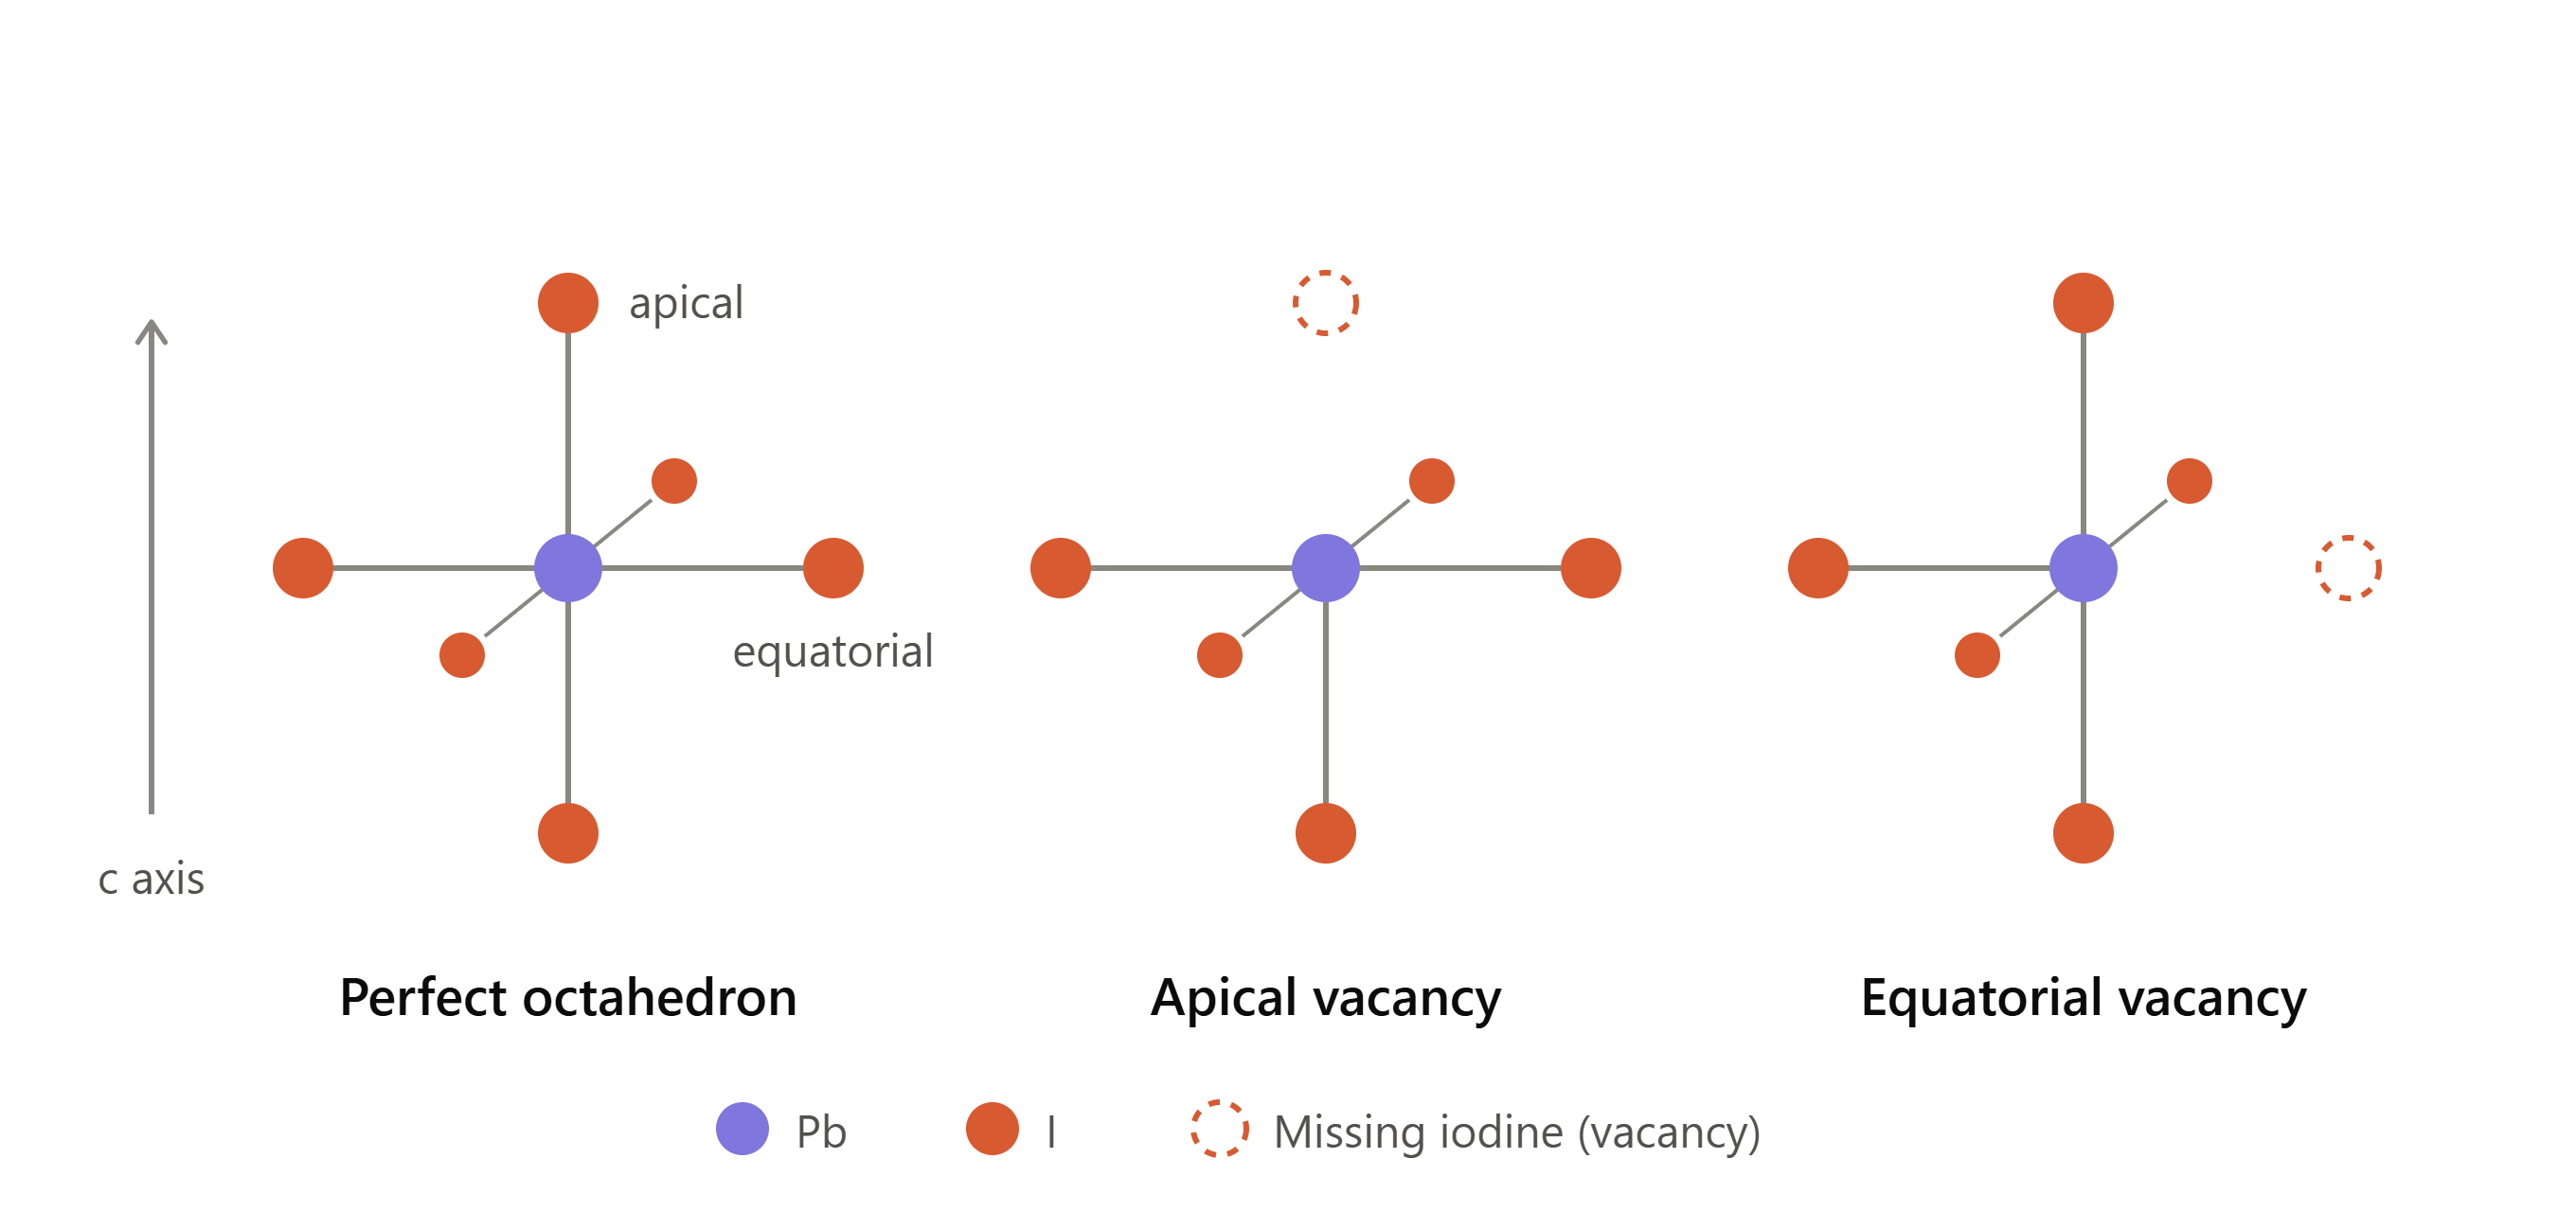
\includegraphics[width=0.85\linewidth]{iodine_vacancy_sites_apical_vs_equatorial.png}
  \caption{Apical (4c) and equatorial (8d) iodine sites of the PbI$_6$ octahedron in \gcpi{}, and the corresponding vacancies.}
  \label{fig:sites}
\end{figure}

\citet{Arber2025} reported one barrier for each of these three path types, with 0.34~eV for 8d--8d hops, 0.35~eV for 8d--4c hops and 0.77~eV for 4c--4c hops. \citet{Zhang2025} calculated two paths and obtained barriers near 0.5~eV. The tilt, however, also makes hops of the same type inequivalent. Two 8d--8d hops can differ in length and in the arrangement of the surrounding octahedra, so the symmetry of the crystal allows several distinct barriers for each path type. \citet{Smolders2024} calculated every symmetrically distinct hop of the halide and cesium vacancies in orthorhombic CsPbBr$_3$, which has the same $Pnma$ structure. Under biaxial strain, the barriers rose or fell depending on the hop and on the strained plane, often non-monotonically. The diffusivity therefore changed differently along each crystal axis, and strain made the diffusion anisotropic. No comparable hop-resolved study exists for \gcpi{}.

\section{Summary and open questions}
\label{sec:summary}

The literature establishes the following points.
\begin{enumerate}
  \item Record perovskite cells use mixed hybrid compositions, whereas all-inorganic mixed-halide perovskites trade some efficiency for thermal stability and suit the top cell of tandem devices.
  \item \gcpi{} is metastable with respect to $\delta$-\cpi{}, and in-plane tensile strain keeps films in the black phase.
  \item Tensile strain lowers the migration barrier of halide vacancies, while compression raises it.
  \item The two iodine sites of \gcpi{} and the inequivalent hops between them allow strain to change each barrier differently.
\end{enumerate}

Four questions remain open. The first concerns whether strain changes the energy difference between $\gamma$ and $\delta$ enough to explain the stabilization, or whether the stabilization must be kinetic. The second concerns how strain changes the formation energy of the positively charged iodine vacancy and the charge transition level. The third concerns which hops carry the vacancy transport in \gcpi{} and how strain changes each barrier and the diffusivity tensor. The fourth concerns whether the charge state of the vacancy changes these conclusions. This thesis addresses these questions for \gcpi{} with DFT. \cpi{} is the end member of the CsPb(I,Br)$_3$ series and shares the $Pnma$ structure with CsPbBr$_3$, so the methods and results also serve as a template for the other all-inorganic halide perovskites.
